% ACL paper: what makes a good rollout for on-policy post-training (rewrite 2026-11-15, storyline papers/apod-story.md v4).
% Evidence: experiments/p2b-analysis/* built from outputs/runs_results/p2b/ (2B selection program, seed 1; seed 2 partial).
% Previous version (aligned-band headline) is in git at b7fc097. Keep the % src: comments.
\documentclass[11pt]{article}

% Change "review" to "final" to generate the final (sometimes called camera-ready) version.
% Change to "preprint" to generate a non-anonymous version with page numbers.
\usepackage[review]{acl}

% Standard package includes
\usepackage{times}
\usepackage{latexsym}

% For proper rendering and hyphenation of words containing Latin characters (including in bib files)
\usepackage[T1]{fontenc}

% This assumes your files are encoded as UTF8
\usepackage[utf8]{inputenc}

% This is not strictly necessary, and may be commented out,
% but it will improve the layout of the manuscript,
% and will typically save some space.
\usepackage{microtype}

% This is also not strictly necessary, and may be commented out.
% However, it will improve the aesthetics of text in
% the typewriter font.
\usepackage{inconsolata}

%Including images in your LaTeX document requires adding
%additional package(s)
\usepackage{graphicx}

% Added for this paper
\usepackage{booktabs}
\usepackage{amsmath}
\usepackage{amssymb}
\usepackage{multirow}
\usepackage{xcolor}
\usepackage{longtable}
\usepackage{array}
\newcolumntype{P}[1]{>{\raggedright\arraybackslash}p{#1}}

\newcommand{\ci}[2]{\,[{#1},\,{#2}]}
\newcommand{\pts}{\,pts}
\newcommand{\accfin}{acc$|$fin}
\newcommand{\pending}[1]{\textcolor{red}{[pending: #1]}}

\title{What Makes a Good Rollout for On-Policy Post-Training?\\Choose the Question, Not the Answer}

\author{First Author \\
  Affiliation / Address line 1 \\
  \texttt{email@domain} \\\And
  Second Author \\
  Affiliation / Address line 1 \\
  \texttt{email@domain} \\}

\begin{document}
\maketitle

% STATUS (2026-11-15): seed 1 of 3 for every arm; seed 2 of the question-KL group to step 45. Numbers marked
% "% src: ... s1" come from experiments/p2b-analysis/{s1_analysis.json, curve_ci.json, signals.json, finish_decomp.txt}
% (built from outputs/runs_results/p2b/, pulled from the VM). Claims we expect to change with seeds 2-3 are listed in
% papers/apod-story.md §5. Repo -> paper names: kl_high/mid/low = rollout KL high/middle/low; ent_top4 = rollout entropy
% high; qkl_high/mid/low = question KL high/middle/low; t_right_s_wrong / both_right / mixed / both_wrong = correctness
% buckets; random = random. The earlier MidAlign runs are the pilot study (Appendix B).
\begin{abstract}
On-policy post-training lets a stronger teacher correct a small model's own answers token by token.
It works, but it is expensive: every answer is a long generation that the teacher has to read, and the usual recipe trains on whatever was sampled.
We wanted to know what makes a rollout worth training on.
We started from three properties that sound right: the answer is correct, it is aligned with the teacher's distribution (neither too close nor too far in reverse KL), and the student is uncertain about it.
We turned each into a rule for choosing questions and answers, and trained a Qwen3.5-2B student with a Qwen3.5-9B teacher under one budget.
At the question level both alignment and correctness mattered. Training on the questions where teacher and student disagree most gained 1.7 points on MATH-500 over random selection, while the most aligned questions lost 1.9 and questions neither model solves lost 1.7. % src: curve_ci.json qkl_high +1.69, qkl_low -1.93, both_wrong -1.71
Choosing answers did not help at all: every answer-level rule, including the aligned middle band we expected to win, stayed within 0.4 points of random. % src: curve_ci.json kl_high -0.34, kl_mid -0.30, kl_low +0.25, ent_top4 -0.06
So filter out questions nobody can solve, prefer questions where teacher and student disagree, and do not spend effort choosing among answers.
\end{abstract}

%=====================================================================
\section{Introduction}
\label{sec:intro}

On-policy post-training is one of the simplest ways to make a small reasoning model better.
The student writes its own answer, a stronger frozen teacher scores every token, and the student moves toward what the teacher would have said by minimizing reverse KL \citep{agarwal2024gkd,gu2024minillm,lu2025opd}.
It is now a standard step for small reasoning models \citep{yang2025qwen3}.

The problem is cost.
A reasoning answer runs to thousands of tokens and the teacher has to read every one of them \citep{ko2024distillm,zhang2026fullrollouts}.
In our setting the student's first training answers average about 7,900 tokens, and scoring them with the teacher takes longer than training on them (\S\ref{sec:cost}). % src: p2b-rollout-s1 metrics.jsonl random step 0 rollouts mean_response_length 7933.8; wall_clock medians oracle 14.9 min vs train 10.9 min
Still, the usual recipe trains on whatever was sampled.
We believe some answers teach more than others, and if we knew which, we could spend the teacher's compute there.

So we asked a simple question: what makes a rollout good for training?
Three answers come up again and again, and all three sound right.
\begin{enumerate}
\setlength\itemsep{0pt}
\item \emph{Correctness.} Train where the teacher is right and the student is wrong; questions nobody solves teach nothing.
\item \emph{Distributional alignment.} Train on answers that are neither too close to the teacher (nothing to learn) nor too far from it (too much to absorb). We believed this one ourselves after a pilot study (\S\ref{sec:pilot}).
\item \emph{Uncertainty.} Train where the student is unsure, as in active learning \citep{settles2009active,kung2023active}.
\end{enumerate}
Each property can be used in two places: to choose which questions get a training slot, and to choose which of a question's answers we keep (Figure~\ref{fig:method}).

We tested all of them in one controlled program (\S\ref{sec:setup}).
Every arm trains the same Qwen3.5-2B student with the same frozen Qwen3.5-9B teacher for 60 steps on 480 answers per refresh, drawn from one shared pool of OpenThoughts math questions, and only the selection rule changes.
That gives eleven rules, each compared with random selection (Table~\ref{tab:arms}).
Here is what we found.
\begin{enumerate}
\setlength\itemsep{0pt}
\item \textbf{Question alignment matters, in the direction we did not expect.} The third of questions where teacher and student disagree most gains 1.69 points over random, and the most aligned third loses 1.93 (\S\ref{sec:question}). A second seed repeats the ordering. % src: curve_ci.json qkl_high +1.69, qkl_low -1.93; p2b-qkl-s2 metrics.jsonl
\item \textbf{Question correctness matters, mostly as a filter.} Questions neither model solves lose 1.71 points, while questions the teacher solves gain 0.80 to 0.90 whether or not the student does (\S\ref{sec:question}). % src: curve_ci.json t_right_s_wrong +0.90, both_right +0.80, both_wrong -1.71
\item \textbf{Choosing answers does not matter.} Keeping the high, middle or low KL third of a question's answers, or its most uncertain ones, stays within 0.4 points of random (\S\ref{sec:rollout}). This is the opposite of what we expected going in. % src: curve_ci.json
\end{enumerate}

Why would the question matter and the answer not?
We believe it comes down to what the loss sees.
Reverse KL never sees whether the final answer is right; it sees how far the student's next-token distribution is from the teacher's.
Question KL measures exactly that, and the answers to one question share most of it (\S\ref{sec:analysis}).

\begin{figure*}[t]
  \centering
  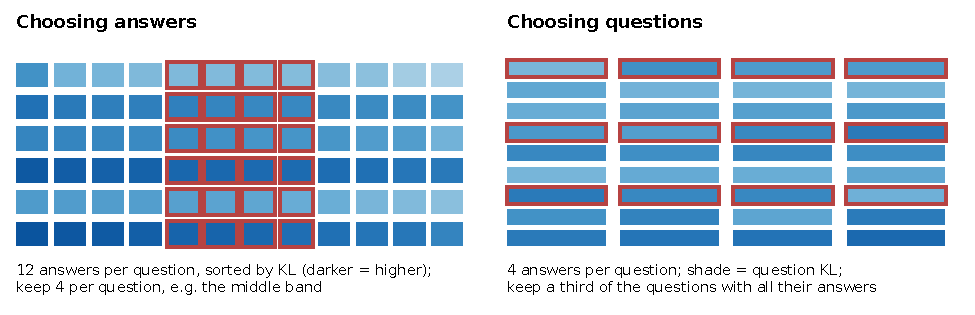
\includegraphics[width=\textwidth]{figures/p2b_method.pdf}
  \caption{The two places a selection rule can act. Left: sample 12 answers per question, rank them by a score (here reverse KL) and keep 4 per question. Right: sample 4 answers for each of 360 questions, score each question by the mean over its answers, and keep a third of the questions with all their answers. Every arm trains on 480 answers per refresh. Schematic; shades are illustrative.} % src: figures/p2b_method.pdf (schematic, no data values)
  \label{fig:method}
\end{figure*}

%=====================================================================
\section{Related Work}
\label{sec:related}

\paragraph{On-policy post-training.}
GKD and MiniLLM train the student on its own samples with reverse KL \citep{agarwal2024gkd,gu2024minillm}, now a standard step for small reasoning models \citep{yang2025qwen3,lu2025opd}.
Recent work asks when it works \citep{li2026rethinking,fu2026revisiting}, studies its entropy structure \citep{yang2026shape,jin2026eopd} and the gap to much stronger teachers \citep{li2025smallmodels}, and asks whether full rollouts are needed \citep{zhang2026fullrollouts}.

\paragraph{Data selection in on-policy post-training.}
Two recent studies are closest to ours.
\citet{hou2026whatmatters} find that hard questions help most, even ones beyond the teacher's reach, and that eight hard questions can match a 17K-question set.
\citet{wang2026beyondprompt} compare prompt selectors, including a sampled teacher-student reverse-KL score, and find that none consistently beats uniform random sampling.
On correctness, \citet{li2026everycoin} report that training difficulty barely matters and that problems the teacher never solves are still useful, while \citet{yang2026correcting} find that training only on problems the student fails lowers accuracy in all eight of their configurations.
These results pull in different directions.
We test all of them in one design, at the level of questions and of answers, against the same random baseline.

\paragraph{Selection more broadly.}
Active learning trains on the examples a model is least sure about \citep{settles2009active,kung2023active}.
Curricula and data selection often target examples that are neither too easy nor too hard \citep{mindermann2022rholoss,tzannetos2023proximal,foster2025learnability,liu2026sweetspot}, and RL with verifiable rewards selects tokens, prompts and rollouts \citep{lin2024rho1,wang2025beyond8020,yu2025dapo,xu2025pods}.
Random selection remains a strong baseline \citep{xia2024random}, and selector comparisons can flip with the learning rate \citep{zhu2026sharedlr}.
Math benchmarks are sensitive to seeds \citep{hochlehnert2025sober,miller2024errorbars}, so every comparison here is repeated over three training seeds.

%=====================================================================
\section{Where We Started}
\label{sec:pilot}

Our starting hypothesis came from a pilot.
We ranked each question's 12 answers by reverse KL and trained on one third, at a constant learning rate of $2\times10^{-5}$ with Adam reset every round.
In one run the middle third reached 47.45\% on MATH-500 against 38.80\% for random after 34 steps, and after one round at a 16k budget it led by 3.75 and 3.70 points in two seeds. % src: results_tables.md kl50 step 34 (0.4745, 0.3880); oracle16k/oracle16k_seed2 kl_mid r1 +3.75/+3.70
That looked like a clear win for the aligned middle band.

To be fair, the pilot also showed why it could not be trusted.
Over all ten middle-versus-random checkpoints the mean lead was only 1.20 points, the same configuration on two seeds differed by up to 24 points, and a 100-step run at $3.16\times10^{-6}$ showed no effect (+0.05). % src: critique-results §3.1(5) recomputed +1.20; apod-story v3 Beat 6 (24 pts; MidAlign-long +0.05)
It also compared only answer-level rules.
So we designed the program below to test it properly, next to the other two properties, with one random baseline and a schedule fixed in advance.

%=====================================================================
\section{Setup}
\label{sec:setup}

\subsection{Objective and scores}
Let $\pi_\theta$ be the student, $\pi_T$ the frozen teacher and $y\sim\pi_\theta(\cdot\mid x)$ an answer to question $x$.
The per-token reverse KL, computed exactly over the full vocabulary with the teacher reading the student's tokens, is
\begin{equation}
D_t(y)=D_{\mathrm{KL}}\!\left(\pi_\theta(\cdot\mid x,y_{<t})\,\middle\|\,\pi_T(\cdot\mid x,y_{<t})\right).
\label{eq:dt}
\end{equation}
Training minimizes its token average over the kept answers $S$,
\begin{equation}
\mathcal{L}(\theta)=\frac{1}{\sum_{y\in S}|y|}\sum_{y\in S}\sum_{t=1}^{|y|}D_t(y),
\label{eq:loss}
\end{equation}
with TRL's \texttt{GKDTrainer} ($\beta=1$, $\lambda=0$) \citep{vonwerra2020trl}. % src: p2b-rollout-s1 resolved_config.yaml train.beta 1.0, lmbda 0.0
We score an answer by its mean KL and a question by the mean score of its $n$ answers,
\begin{equation}
s(y)=\frac{1}{|y|}\sum_{t=1}^{|y|}D_t(y),\qquad s(x)=\frac{1}{n}\sum_{i=1}^{n}s(y_i).
\label{eq:score}
\end{equation}
The uncertainty score is the same average of the student's own token entropy, which needs no teacher.
So the alignment score is exactly the quantity the loss will push down.

\subsection{Selection rules}
Every 15 optimizer steps (a \emph{refresh}) the current student samples new answers with vLLM \citep{kwon2023vllm}, the teacher scores all of them, and the arm's rule keeps 480, which is one epoch of 15 steps at an effective batch of 32. % src: resolved_config.yaml refresh_every 15, micro 8 x accum 2 x 2 GPUs; metrics.jsonl: 1440 generated (rollout, qkl), 480 generated (correct), 480 kept (all)
Four refreshes give 60 steps.
Questions are never reused, and arms at the same level start from the same first pool.
\begin{itemize}
\setlength\itemsep{0pt}
\item \emph{Answer-level} arms draw 120 questions and sample 12 answers each, then keep 4 per question: KL ranks 1 to 4, 5 to 8 or 9 to 12, the four with the highest student entropy, or four at random.
\item \emph{Question-alignment} arms draw 360 questions with 4 answers each and keep the high, middle or low third of questions by $s(x)$, with all their answers.
\item \emph{Correctness} arms draw 120 questions from one bucket (\S\ref{sec:bank}) and keep all 4 answers of each, so they sample 480 answers rather than 1,440.
\end{itemize}
Random is the shared baseline: keeping four of twelve at random is the same, in distribution, as sampling four, which is what the usual recipe does.
All arms train on 480 answers per refresh; they differ only in which ones.

\begin{table}[t]
\centering\small
\setlength{\tabcolsep}{4pt}
\begin{tabular}{@{}p{1.75cm}p{2.45cm}p{2.6cm}@{}}
\toprule
Property & Answer level & Question level \\
\midrule
Alignment (KL) & keep KL ranks 1 to 4, 5 to 8, or 9 to 12 of 12 & keep the high, middle or low third of 360 \\
Uncertainty & keep the 4 of 12 with highest entropy & highest-entropy third of 360 (pending, \S\ref{sec:qent}) \\
Correctness & n/a & 4 buckets: teacher right and student wrong, both right, mixed, both wrong \\
None (random) & keep 4 of 12 at random & n/a \\
\bottomrule
\end{tabular}
\caption{The arms. Each trains on 480 answers per refresh for 4 refreshes of 15 steps. Within a question, answers barely differ in correctness (\S\ref{sec:analysis}), so we test correctness only at the question level.} % src: signals.json A_band_props correct 8.3-9.0%
\label{tab:arms}
\end{table}

\subsection{Questions and correctness labels}
\label{sec:bank}
Training questions come from a competition-math set derived from OpenThoughts \citep{zhao2026openthoughtsdata,guha2025openthoughts}.\footnote{\url{https://huggingface.co/datasets/siyanzhao/Openthoughts_math_30k_opsd}}
We sampled 14,500 of its questions and labeled 4,641 of them with four answers from the teacher and four from the base student at the 8k budget. % src: bank-8k/questions.jsonl 14500 rows, 4641 with teacher_grades (checked 2026-11-15)
Every arm draws its questions from these 4,641, in the same order.
A model \emph{solves} a question if at least 3 of its 4 answers are strictly correct and \emph{fails} it if at most 1 is. % src: resolved_config.yaml bank correct_min 3, wrong_max 1
This gives four buckets: both fail (2,387 questions), the teacher solves and the student fails (971), both solve (866), and \emph{mixed}, every other labeled question (417). % src: bank-8k/questions.jsonl bucket counts over the 4,641 labeled (checked 2026-11-15)
Half of the pool is beyond both models at this budget, so a filter on correctness removes a lot.
The student labels come from the base model and are not updated as it trains, while KL and entropy are rescored every refresh.

\subsection{Models and training}
The student is Qwen3.5-2B and the teacher Qwen3.5-9B \citep{qwen2026qwen35_2b,qwen2026qwen35_9b}, both in thinking mode.
Table~\ref{tab:baselines} gives the untrained baselines at our 8k budget.
We chose the 2B because selection can only show up if the student has a lot to learn from the teacher: the 2B sits 34.65 points below the teacher, while the 4B we first planned to use sits only 4.0 points below it, which leaves almost no room for any rule to differ from random.
Answers are sampled at temperature 1.0, top-$p$ 0.95 and top-$k$ 20 with an 8,192-token cap. % src: resolved_config.yaml rollout temperature 1.0, top_p 0.95, top_k 20, max_new_tokens 8192
Training uses bf16, a peak learning rate of $3.16\times10^{-6}$ with 3 warmup steps and cosine decay to a tenth, and keeps Adam state across refreshes, on two A100 80GB GPUs. % src: resolved_config.yaml learning_rate 3.1623e-06, warmup_steps 3, cosine_with_min_lr min_lr_rate 0.1, persist_optimizer true, bf16 true; VM a2-ultragpu-2g

\begin{table}[t]
\centering\small
\begin{tabular}{@{}llr@{}}
\toprule
Model & Role & MATH-500 (\%) \\
\midrule
Qwen3.5-2B & student & 26.50 \\ % src: s1_analysis.json base strict 0.2650
Qwen3.5-4B & considered student & 57.15 \\ % src: HANDOFF.md §5 (4B base MATH-500 @8k strict avg@4 0.5715)
Qwen3.5-9B & teacher & 61.15 \\ % src: outputs/runs/kl50_teacher avg@4 0.6115 at 8192
\bottomrule
\end{tabular}
\caption{Untrained baselines: strict avg@4 on MATH-500 at an 8,192-token budget.}
\label{tab:baselines}
\end{table}

\subsection{Evaluation}
We evaluate all 500 MATH-500 problems \citep{hendrycks2021math,lightman2023verify} with four samples each at the 8k training budget, at steps 0, 15, 30, 45 and 60.
A sample is strict-correct if Math-Verify accepts it \citep{kydlicek2025mathverify} and it contains \texttt{\textbackslash boxed\{\}}.
We report strict avg@4 and pass@4; Appendix~\ref{app:budget} describes how answers that reach the budget behave.
Our summary of an arm is its mean accuracy over steps 15 to 60, minus that of random; Table~\ref{tab:main} also gives every step.
Our pre-registered primary contrast was the middle KL band against random.
For a sense of evaluation noise, the same base model scored 26.50\% and 27.15\% on two sampling seeds. % src: p2b-qkl-s1 vs p2b-qkl-s2 metrics.jsonl step 0 strict 0.265 / 0.2715

\subsection{Where the compute goes}
\label{sec:cost}
Table~\ref{tab:cost} breaks one refresh into its stages.
Teacher scoring of 1,440 answers takes 14.9 minutes, more than the 10.9 minutes of training on the 480 we keep. % src: wall_clock medians p2b-rollout-s1 (n=20): oracle_s 14.9 min, train_s 10.9 min
Student entropy, the score an uncertainty rule needs, takes 3.7 minutes. % src: wall_clock median entropy_s 3.7 min
So a rule that needs the teacher on every candidate pays for it in scoring, not in training.

\begin{table}[t]
\centering\small
\begin{tabular}{@{}lrr@{}}
\toprule
Stage & 1,440 sampled & 480 sampled \\
\midrule
Generation and evaluation & 22.1 & 15.2 \\
Student entropy & 3.7 & 1.3 \\
Teacher scoring (exact KL) & 14.9 & 4.9 \\
Training (15 steps) & 10.9 & 10.2 \\
\bottomrule
\end{tabular}
\caption{Median minutes per refresh. Left: answer-level and question-alignment arms; right: correctness arms. Evaluation is the MATH-500 run at each refresh.} % src: metrics.jsonl wall_clock medians: p2b-rollout-s1 (n=20) 22.1/3.7/14.9/10.9; p2b-correct-s1 (n=16) 15.2/1.3/4.9/10.2
\label{tab:cost}
\end{table}

%=====================================================================
\section{Results}
\label{sec:results}

\begin{table*}[t]
\centering\small
\setlength{\tabcolsep}{5pt}
\begin{tabular}{@{}lrrrrrrrr@{}}
\toprule
 & \multicolumn{4}{c}{Strict avg@4 (\%) at step} & \multicolumn{2}{c}{Avg@4, steps 15 to 60} & \multicolumn{2}{c}{Pass@4, steps 15 to 60} \\
\cmidrule(lr){2-5}\cmidrule(lr){6-7}\cmidrule(lr){8-9}
Arm & 15 & 30 & 45 & 60 & mean & minus random & mean & minus random \\
\midrule
% src: experiments/p2b-analysis/tex_rows.tex (s1_analysis.json, curve_ci.json point estimates); pass@4: experiments/p2b-analysis/pass4_means.txt; step 0 = 26.50 (pass@4 38.4) for every arm
\multicolumn{9}{@{}l}{\emph{Baseline}} \\
\quad Random & 41.90 & 42.15 & 43.15 & 42.85 & 42.51 & n/a & 54.35 & n/a \\
\multicolumn{9}{@{}l}{\emph{Which answer}} \\
\quad KL high & 41.20 & 41.95 & 43.55 & 42.00 & 42.17 & $-$0.34 & 54.85 & +0.50 \\
\quad KL middle & 41.60 & 42.20 & 42.45 & 42.60 & 42.21 & $-$0.30 & 54.70 & +0.35 \\
\quad KL low & 40.70 & 42.80 & 43.80 & 43.75 & 42.76 & +0.25 & 55.05 & +0.70 \\
\quad Entropy high & 41.95 & 41.80 & 42.40 & 43.65 & 42.45 & $-$0.06 & 54.30 & $-$0.05 \\
\multicolumn{9}{@{}l}{\emph{Which question: alignment}} \\
\quad KL high & 42.15 & 44.45 & 45.65 & 44.55 & 44.20 & +1.69 & 56.55 & +2.20 \\
\quad KL middle & 43.70 & 41.60 & 41.55 & 42.50 & 42.34 & $-$0.18 & 55.35 & +1.00 \\
\quad KL low & 39.15 & 40.30 & 42.40 & 40.50 & 40.59 & $-$1.93 & 52.75 & $-$1.60 \\
\multicolumn{9}{@{}l}{\emph{Which question: correctness}} \\
\quad Teacher right, student wrong & 40.10 & 44.85 & 44.50 & 44.20 & 43.41 & +0.90 & 55.95 & +1.60 \\
\quad Both right & 42.25 & 42.75 & 44.10 & 44.15 & 43.31 & +0.80 & 55.55 & +1.20 \\
\quad Mixed & 39.80 & 43.15 & 44.40 & 43.00 & 42.59 & +0.07 & 55.00 & +0.65 \\
\quad Both wrong & 40.70 & 40.55 & 40.75 & 41.20 & 40.80 & $-$1.71 & 53.70 & $-$0.65 \\
\bottomrule
\end{tabular}
\caption{MATH-500 at an 8k budget, seed 1. Every arm starts from the base student (avg@4 26.50\%, pass@4 38.4\%). Differences are in points.}
\label{tab:main}
\end{table*}

\begin{figure}[t]
  \centering
  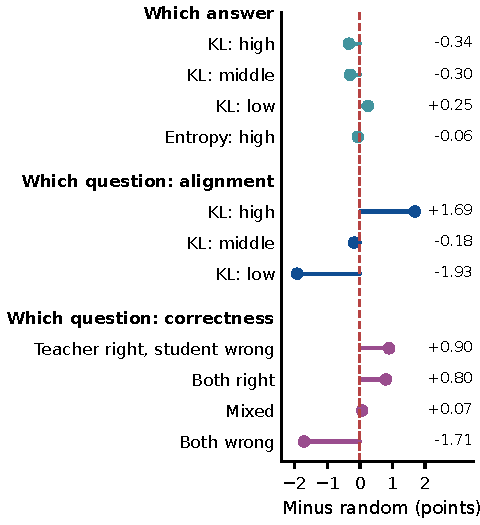
\includegraphics[width=\columnwidth]{figures/p2b_forest.pdf}
  \caption{Each rule minus random, MATH-500 strict avg@4, averaged over steps 15, 30, 45 and 60 (seed 1). Answer-level rules (top) stay near zero; question-level rules (middle, bottom) spread out.} % src: figures/p2b_forest.pdf from curve_ci.json point estimates (make_figures_p2b.py)
  \label{fig:forest}
\end{figure}

\begin{figure*}[t]
  \centering
  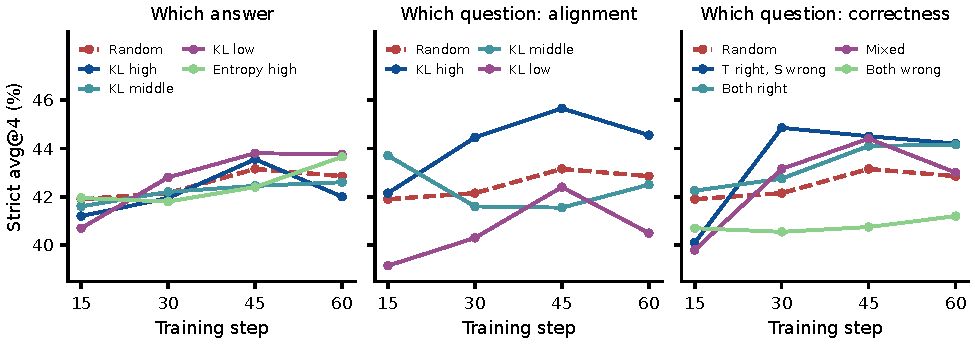
\includegraphics[width=\textwidth]{figures/p2b_curves.pdf}
  \caption{Learning curves for each group of rules, seed 1 (step 0 is 26.50\% for every arm). Random (dashed red) is the same run in every panel.} % src: figures/p2b_curves.pdf from s1_analysis.json
  \label{fig:curves}
\end{figure*}

Training helps every arm: random selection lifts the student from 26.50\% to 42.85\% in 60 steps, closing almost half of the 34.65-point gap to the teacher (Table~\ref{tab:main}). % src: s1_analysis.json random step 0 0.2650 -> step 60 0.4285; (42.85-26.50)/34.65 = 0.47
The question is which rules do better than that.

\subsection{Which answer you keep does not matter}
\label{sec:rollout}

All four answer-level rules end up where random does (Table~\ref{tab:main}, Figure~\ref{fig:forest}).
Over steps 15 to 60 they sit between $-$0.34 and +0.25 points.
The middle KL band, our pre-registered method, is at $-$0.30, so the aligned-band hypothesis from the pilot is not supported in this design. % src: curve_ci.json kl_mid
Keeping the most uncertain answers, the classic active-learning rule, is at $-$0.06.
At no single step does an answer-level rule differ from random by more than 1.2 points (Figure~\ref{fig:curves}, left), and on pass@4 they stay within 0.7 points. % src: analyze_s1.py per-step diffs vs random, max |diff| 1.20 (kl_low step 15); pass4_means.txt answer-level -0.05..+0.70

\subsection{Which question you train on does}
\label{sec:question}

Question-level rules spread over 3.6 points, six times the spread of the answer-level rules (Figure~\ref{fig:forest}). % src: curve_ci.json qkl_high +1.69 - qkl_low -1.93 = 3.62; answer-level +0.25 - (-0.34) = 0.59

\paragraph{Alignment.}
By question alignment the order is monotone, and it runs the other way from our hypothesis: the high third gains 1.69 points, the middle third $-$0.18 and the low third loses 1.93. % src: curve_ci.json
Pass@4 shows the same order (+2.20, +1.00, $-$1.60), so training on high-KL questions does not trade coverage for accuracy. % src: pass4_means.txt qkl_high +2.20, qkl_mid +1.00, qkl_low -1.60
The high third leads the middle third from step 30 on (Figure~\ref{fig:curves}, middle).
A second training seed, with new questions, repeats it (Table~\ref{tab:seed2}): high minus middle is +1.61 points against +1.86 in seed 1. % src: p2b-qkl-s2.metrics.jsonl (pulled 2026-11-15) high 43.00/43.60/43.90/44.30, mid 40.30/42.60/42.85/42.60; s1 means 44.20 vs 42.34

\begin{table}[t]
\centering\small
\setlength{\tabcolsep}{4pt}
\begin{tabular}{@{}llrrrrr@{}}
\toprule
Seed & Question KL & 15 & 30 & 45 & 60 & Mean \\
\midrule
1 & high & 42.15 & 44.45 & 45.65 & 44.55 & 44.20 \\
1 & middle & 43.70 & 41.60 & 41.55 & 42.50 & 42.34 \\
2 & high & 43.00 & 43.60 & 43.90 & 44.30 & 43.70 \\ % src: p2b-qkl-s2.metrics.jsonl qkl_high
2 & middle & 40.30 & 42.60 & 42.85 & 42.60 & 42.09 \\ % src: p2b-qkl-s2.metrics.jsonl qkl_mid
\bottomrule
\end{tabular}
\caption{Question-alignment arms in two training seeds with different questions (strict avg@4, \%). The low third and the third seed are still running.}
\label{tab:seed2}
\end{table}

\paragraph{Correctness.}
Questions the teacher solves and the student fails gain 0.90 points, questions both solve gain 0.80, mixed questions do nothing and questions both fail lose 1.71. % src: curve_ci.json
The two buckets the teacher solves are within 0.10 points of each other, so in this seed it matters little whether the student also solves them.
The clearest effect is a filter: drop the questions nobody can solve.
Questions that both models fail also hurt in our pilot, which used a different design: a fixed set of 800 questions over 100 steps ($-$2.59 points; Appendix~\ref{app:pilot}). % src: papers/apod-story.md v3 Beat 7 (r1 both-wrong -2.59 pooled)
This agrees with \citet{yang2026correcting} and disagrees with \citet{li2026everycoin}; we come back to it in \S\ref{sec:analysis}.

\subsection{Can the student pick its own questions?}
\label{sec:qent}

Question alignment needs a teacher pass on every candidate question, which Table~\ref{tab:cost} shows is the expensive part.
The student's own uncertainty may be enough.
Ranked by the student's mean entropy over their 4 answers, questions order almost as they do by KL (Spearman 0.92 to 0.94 in every pool we scored), and 101 to 109 of the 120 most uncertain questions fall in the high-KL third, against 40 by chance. % src: experiments/p2b-analysis/qent_verify.txt (8 qkl pools, seeds 1-2, rounds 0-3; entropy-stage scores)
Training on the most uncertain third of questions gives \pending{qent\_high minus random} points, against +1.69 for the high-KL third. % TODO: fill from p2b-qent-s{1,2,3} (outputs/prompts/qent-experiment-prompt.md)
A related rule in our pilot, which ranked the whole bank once and kept its 800 most uncertain questions, lost 1.38 points (Appendix~\ref{app:pilot}). % src: notes/apod-lit-review.md §4.3 (r3 uncertain -1.38)

%=====================================================================
\section{Why the Question Matters and the Answer Does Not}
\label{sec:analysis}

\begin{figure*}[t]
  \centering
  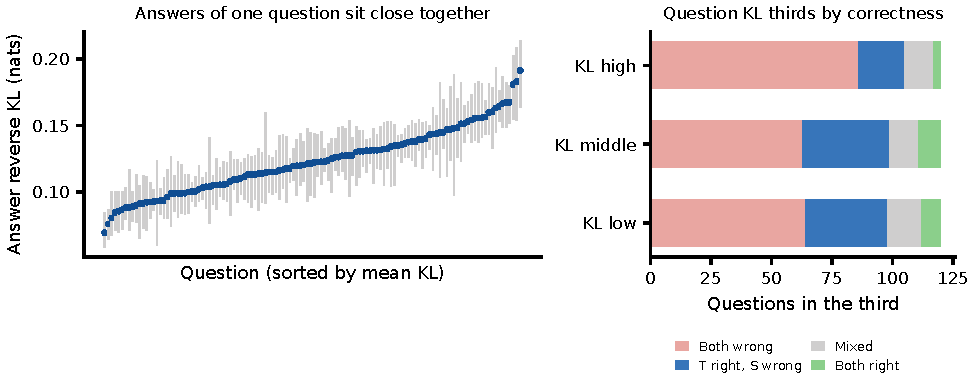
\includegraphics[width=\textwidth]{figures/p2b_signals.pdf}
  \caption{What the signals measure, in the base student's first pools (seed 1). Left: answer KL for 120 questions with 12 answers each; dots are question means, gray bars the range of a question's answers. Right: the correctness buckets inside each third of 360 questions ranked by question KL.} % src: figures/p2b_signals.pdf from p2b_rollouts_compact.jsonl (make_figures_p2b.py); thirds 86/19/12/3, 63/36/12/9, 64/34/14/8
  \label{fig:signals}
\end{figure*}

\begin{table}[t]
\centering\small
\setlength{\tabcolsep}{3.2pt}
\begin{tabular}{@{}lrrrrr@{}}
\toprule
 & KL & Ent. & Stud. & Teach. & Both \\
 & (nats) & & correct & pass & wrong \\
\midrule
\multicolumn{6}{@{}l}{\emph{Answer KL bands (120 q.\ $\times$ 4 each)}} \\
% src: signals.json A_band_props (round 0, p2b-rollout-s1 random pool, 1,440 answers)
\quad high (1 to 4) & 0.134 & 0.57 & 9.0\% & n/a & n/a \\
\quad middle (5 to 8) & 0.123 & 0.54 & 8.3\% & n/a & n/a \\
\quad low (9 to 12) & 0.112 & 0.49 & 8.8\% & n/a & n/a \\
\multicolumn{6}{@{}l}{\emph{Question KL thirds (120 q.\ each)}} \\
% src: signals.json B_thirds (round 0, p2b-qkl-s1 pool, 360 questions); teacher pass from bank-8k (9B, 4 answers)
\quad high & 0.148 & 0.66 & 4.4\% & 24.8\% & 86 \\
\quad middle & 0.120 & 0.51 & 10.0\% & 40.8\% & 63 \\
\quad low & 0.095 & 0.40 & 9.4\% & 39.4\% & 64 \\
\bottomrule
\end{tabular}
\caption{What each rule picks from the base student's first pool. Ent.: student token entropy. Stud.\ correct: strict accuracy of the student's answers. Teach.\ pass: the 9B's pass rate on the same questions. Both wrong: questions in that bucket.}
\label{tab:signals}
\end{table}

\paragraph{The answers to one question are nearly the same example.}
In the base student's first pool, 84.6\% of the variance in answer KL lies between questions (Figure~\ref{fig:signals}, left). % src: signals.json A_between_frac 0.846
The three KL bands of a question differ by about 9\% in mean KL and not at all in correctness (8.3 to 9.0\%; Table~\ref{tab:signals}). % src: signals.json A_band_props kl 0.134/0.123/0.112, correct 0.090/0.083/0.088
Picking a band therefore changes the training signal very little, which is what Table~\ref{tab:main} shows.
Entropy behaves the same way: within a question it ranks answers much like KL (Spearman 0.69), and the four most uncertain answers overlap the four highest-KL ones 2.63 times out of 4, against 1.33 by chance. % src: signals.json A_within_spear_kl_sent 0.692, A_overlap_enttop4_klhigh 2.625
Answer KL is not a length proxy either; its within-question correlation with length is 0.20. % src: signals.json A_within_spear_kl_len 0.199 (18 questions with length variation)

\paragraph{Question alignment is not correctness.}
We expected the best questions to be the ones where the teacher knows more. They are not.
The high-KL third is mostly questions both models fail (86 of 120; Figure~\ref{fig:signals}, right), and the teacher answers only 24.8\% of its own attempts correctly there, against about 40\% in the other two thirds (Table~\ref{tab:signals}). % src: signals.json B_thirds
Across the 360 questions, question KL barely correlates with the teacher's pass rate (Spearman $-$0.15) or the student's ($-$0.11). % src: signals.json B_spear_qkl_teacherpass -0.147, B_spear_qkl_studentpass -0.108
What it does track is uncertainty in both models: student entropy is 0.66 in the high third and 0.40 in the low third, and teacher entropy 0.58 and 0.34. % src: signals.json B_thirds sent/tent

\paragraph{What each arm actually trained on.}
Table~\ref{tab:trained} shows the 480 answers each arm trained on per refresh.
The high-KL arm keeps training on high-KL questions as the student improves: 0.122 nats per token in its last three refreshes against 0.077 for the low arm. % src: s1_analysis.json selected kl per refresh qkl_high 0.1216/0.1224/0.1220, qkl_low 0.0773/0.0775/0.0742
The both-wrong arm, in contrast, trained on answers with ordinary KL (0.105 nats, random 0.104), only 11.4\% of them correct. % src: tex_rows.tex trained-set rows both_wrong 0.105, correct 11.4; random 0.104
So high-KL questions and both-wrong questions overlap but are not the same thing: a hard question helps when the teacher disagrees with the student a lot, and hurts when it does not.
This may be why the literature disagrees: hard questions help \citep{hou2026whatmatters}, but a bucket of failed questions on its own does not \citep{yang2026correcting}.
Training on correct answers is not enough either: the both-right arm trained on answers that were 95.4\% correct and gained 0.80 points, less than the high-KL arm, whose answers were 23.3\% correct. % src: tex_rows.tex both_right correct 95.4, qkl_high correct 23.3; curve_ci.json both_right +0.80, qkl_high +1.69

\begin{table}[t]
\centering\small
\setlength{\tabcolsep}{4pt}
\begin{tabular}{@{}lrrr@{}}
\toprule
Arm & KL (nats) & Entropy & Correct (\%) \\
\midrule
% src: experiments/p2b-analysis/tex_rows.tex (s1_analysis.json "selected", mean over 4 refreshes)
Random & 0.104 & 0.387 & 25.5 \\
\multicolumn{4}{@{}l}{\emph{Which answer}} \\
\quad KL high & 0.114 & 0.422 & 25.3 \\
\quad KL middle & 0.104 & 0.390 & 25.9 \\
\quad KL low & 0.095 & 0.353 & 26.0 \\
\quad Entropy high & 0.112 & 0.434 & 25.7 \\
\multicolumn{4}{@{}l}{\emph{Which question: alignment}} \\
\quad KL high & 0.129 & 0.496 & 23.3 \\
\quad KL middle & 0.101 & 0.370 & 27.7 \\
\quad KL low & 0.081 & 0.291 & 28.2 \\
\multicolumn{4}{@{}l}{\emph{Which question: correctness}} \\
\quad T right, S wrong & 0.104 & 0.383 & 48.5 \\
\quad Both right & 0.094 & 0.329 & 95.4 \\
\quad Mixed & 0.100 & 0.374 & 48.1 \\
\quad Both wrong & 0.105 & 0.395 & 11.4 \\
\bottomrule
\end{tabular}
\caption{The 480 answers each arm trained on per refresh, averaged over the four refreshes: mean reverse KL, student entropy and strict accuracy of the answers.}
\label{tab:trained}
\end{table}

\paragraph{What we think is happening.}
Reverse-KL post-training moves the student wherever its next-token distribution differs from the teacher's (Eq.~\ref{eq:loss}), and it never sees whether the final answer is right.
The signal a question offers is how much disagreement it carries, which is question KL.
A low-KL question gives the student little to move toward, so its refresh is mostly wasted.
Answers to one question share that question's disagreement, so choosing among them moves almost nothing.
High-KL questions are those where both models are least certain, and we believe the teacher's corrections there show the student how to reason through that uncertainty.
We have not yet located which tokens carry the KL in these answers; that is the most direct test of this reading (\S\ref{sec:discussion}).

%=====================================================================
\section{Discussion}
\label{sec:discussion}

So, what makes a rollout good for training? For a small student on a tight budget, mostly the question it comes from.
In practice:
\begin{enumerate}
\setlength\itemsep{0pt}
\item filter out questions neither model can solve;
\item among the rest, prefer questions where teacher and student disagree most, and skip those where they already agree;
\item do not spend effort choosing among a question's answers, by KL or by entropy.
\end{enumerate}
We expected the aligned middle band of answers to win, and we were wrong.

We expect the descriptive findings to hold as seeds come in, since they are properties of the data rather than of one training run: answers to one question are nearly the same example, and question alignment and correctness measure different things.
The sizes of the question-level effects are what the next runs will pin down:
\begin{enumerate}
\setlength\itemsep{0pt}
\item seeds 2 and 3 for every arm, now running, to measure training noise;
\item a best-checkpoint pick on 200 held-out training-distribution questions, as pre-registered;
\item re-evaluation at a 16k or 32k budget, to check that the ranking holds with more room to think;
\item a token-level map of where the KL sits in high-KL questions, which needs no new training.
\end{enumerate}

%=====================================================================
\section*{Limitations}

\begin{enumerate}
\setlength\itemsep{0pt}
\item Most numbers in Table~\ref{tab:main} come from one training seed; only the high and middle question-alignment arms have a second. In our pilot, training noise was larger than most effects (Appendix~\ref{app:pilot}). Runs 1 and 2 address this.
\item We train and evaluate at one 8k budget, which shapes what accuracy measures (Appendix~\ref{app:budget}); run 3 addresses this.
\item We test one model pair, one training set, one learning rate and MATH-500 only. Selector comparisons can change with the learning rate \citep{zhu2026sharedlr}.
\item The question-alignment rule needs a teacher pass on every candidate question, so it saves training steps but not scoring (\S\ref{sec:cost}, \S\ref{sec:qent}).
\item The correctness buckets use labels from the base student, which go stale as it trains, while the KL arms rescore every refresh.
\end{enumerate}

\section*{Ethics and Reproducibility Statement}

We use public models (Qwen3.5-2B and -9B, Apache-2.0) and data (MATH-500; the OpenThoughts-derived set, whose card lists no license), and see no risks beyond those of the base models.
We release code, configurations, evaluation shards, reverse-KL and entropy scores and training logs for every run.

\bibliography{refs}

%=====================================================================
\appendix

\section{Pass@4 by Step}
\label{app:full}

\begin{table}[ht]
\centering\small
\setlength{\tabcolsep}{4pt}
\begin{tabular}{@{}lrrrr@{}}
\toprule
Arm & 15 & 30 & 45 & 60 \\
\midrule
% src: experiments/p2b-analysis/s1_analysis.json curves[arm][step].pass4; step 0 = 38.4 for every arm
Random & 53.8 & 54.2 & 55.0 & 54.4 \\
\multicolumn{5}{@{}l}{\emph{Which answer}} \\
\quad KL high & 54.0 & 54.0 & 55.8 & 55.6 \\
\quad KL middle & 55.4 & 54.2 & 54.6 & 54.6 \\
\quad KL low & 53.6 & 55.0 & 56.2 & 55.4 \\
\quad Entropy high & 54.0 & 54.0 & 54.4 & 54.8 \\
\multicolumn{5}{@{}l}{\emph{Which question: alignment}} \\
\quad KL high & 55.6 & 56.2 & 57.6 & 56.8 \\
\quad KL middle & 56.4 & 54.6 & 55.6 & 54.8 \\
\quad KL low & 52.0 & 53.4 & 52.6 & 53.0 \\
\multicolumn{5}{@{}l}{\emph{Which question: correctness}} \\
\quad T right, S wrong & 53.8 & 56.6 & 57.2 & 56.2 \\
\quad Both right & 53.8 & 55.2 & 57.2 & 56.0 \\
\quad Mixed & 53.4 & 55.6 & 56.0 & 55.0 \\
\quad Both wrong & 53.4 & 54.2 & 54.0 & 53.2 \\
\bottomrule
\end{tabular}
\caption{MATH-500 strict pass@4 (\%) by step, seed 1.}
\label{tab:pass4}
\end{table}

\section{Pilot Study}
\label{app:pilot}

The answer-level pilot runs are summarized in \S\ref{sec:pilot}. The short runs used a constant learning rate of $2\times10^{-5}$ and the 100-step run $3.16\times10^{-6}$; selector verdicts can change with the learning rate \citep{zhu2026sharedlr}, which may explain part of the difference from this program.
In the pilot's question-selection runs, which trained on a fixed set of 800 questions for 100 steps, questions both models fail lost 2.59 points and the 800 most uncertain questions lost 1.38. % src: apod-story v3 Beat 7 (r1 both_wrong -2.59 pooled); notes/apod-lit-review.md §4.3 (r3 uncertain -1.38)
The pilot also showed the effect described in Appendix~\ref{app:budget}: finished answers were correct 98 to 100\% of the time. % src: apod-story v3 Beat 5

\section{Answers That Reach the Budget}
\label{app:budget}

At an 8k budget the base 2B finishes only 20.5\% of its MATH-500 answers, and every one of those 410 finished answers is correct. % src: eval_rows base: fin 410, strict|fin 1.000
Its errors are answers that run out of budget.
This stays true after training: in all 49 evaluations, finished answers are correct at least 99.4\% of the time. % src: s1_analysis.json min acc_fin 0.9936 (qkl_high step 30)
Random selection lifts accuracy from 26.50\% to 42.85\% and the finish rate from 20.5\% to 36.8\%, and across the 48 trained checkpoints accuracy tracks the finish rate with $r=0.80$ (Figure~\ref{fig:finish}). % src: finish_decomp.txt base->random60 +16.35, finish 20.5->36.8; make_figures_p2b.py r(trained, n=48)=0.798
So ``accuracy'' here mostly means ``problems solved within the budget'', and the arms differ mainly in how often they finish.

The differences between arms show up the same way.
Splitting each contrast into a finish-rate part and a remainder, the finish rate accounts for +2.03 of the high-KL third's +1.69 and $-$1.98 of the low third's $-$1.93. % src: finish_decomp.txt qkl_high +2.03, qkl_low -1.98
One arm breaks the pattern: questions both models solve gain through answers that are capped but already contain the boxed answer ($+$1.91 points), not through finishing ($-$1.11). % src: finish_decomp.txt both_right d_from_finish -1.11, d_from_capped +1.91
The trained-on answers were mostly capped as well: 87.6\% for random, 89.8\% for the high-KL arm and 99.0\% for both-wrong. % src: tex_rows.tex trained-set trunc column random 87.6, qkl_high 89.8, both_wrong 99.0

\begin{figure}[t]
  \centering
  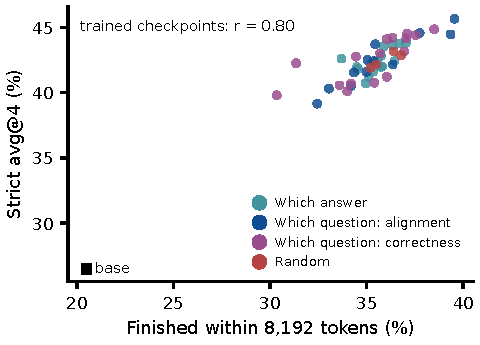
\includegraphics[width=\columnwidth]{figures/p2b_finish.pdf}
  \caption{Strict accuracy against finish rate for every arm and step (48 trained checkpoints, seed 1) and the base model. Finished answers are correct at least 99.4\% of the time, so accuracy mostly measures finishing.} % src: figures/p2b_finish.pdf; s1_analysis.json
  \label{fig:finish}
\end{figure}

Reasoning models are known to overthink \citep{chen2024overthinking,fatemi2025concise}, a termination mismatch can inflate length in on-policy distillation \citep{yang2026eos}, and model rankings change with the token budget \citep{desouza2026budget}, which is why run 3 re-evaluates at a longer budget.

\section{Data and Contamination}
\label{app:data}

The training pool is the OpenThoughts-derived set of \S\ref{sec:bank}: 14,500 sampled questions, 4,641 of them labeled, plus 200 further questions held out for checkpoint selection. % src: bank-8k/questions.jsonl 14500 lines, 4641 labeled; apod/datasets/load.py otval200
Our earlier contamination check found no evaluation problem with a duplicate in the pool that was ever trained on. % src: notes/apod-critique-data.md §4

\end{document}
